\begin{exercice}
Chercher les sinus, cosinus et tangentes des angles suivants :
\begin{multicols}{2}
 \begin{enumerate}
 \item $45^\circ$
 \item $22^\circ$
 \item $48^\circ$
 \item $120^\circ$
 \end{enumerate}
\end{multicols}
\end{exercice}

\begin{exercice}
Chercher les angles dont tu connais la valeur du sinus :
\begin{multicols}{2}
\begin{enumerate} 
\item $0.743144826$
\item $0.906307788$
\item $0.999847696$
\item $0.017452407$
\end{enumerate}
\end{multicols}
\end{exercice}

\begin{exercice}
Chercher les angles dont tu connais la valeur du cosinus :
\begin{multicols}{2}
\begin{enumerate}
\item $0.4539906$
\item $0.034899496$
\item $0.848048096$
\item $0.999390827$
\end{enumerate}
\end{multicols}
\end{exercice}

\begin{exercice}
Chercher les angles dont tu connais la valeur de la tangente :
\begin{multicols}{2}
\begin{enumerate}
\item $0.531709431$
\item $0.017455064$
\item $57.28996163$
\item $4.704630109$
\end{enumerate}
\end{multicols}
\end{exercice}

\begin{exercice}
Tracer un triangle ABC, rectangle en A avec $\overline{AB}$ = 6 cm et $\overline{BC}$ = 12 cm. Calculer la mesure de l’angle B, en degrés. 
\end{exercice}

\begin{exercice}
Tracer un triangle ABC, rectangle en A avec $\overline{AB}$ = 4 cm et l’angle $C = 43^\circ$. Calculer la mesure du côté AC, arrondie au mm près.
\end{exercice}

\begin{exercice}
L’hypoténuse d’un triangle mesure 10 m; l’un des angles mesure $40^\circ$. Calculer la longueur des deux autres côtés du triangle.
\end{exercice}

\begin{exercice}
Une échelle, appuyée contre un mur vertical, forme avec le mur un angle de $3^\circ$. Le pied de l’échelle est distant de 3 m du mur. A quelle hauteur du mur l’échelle est-elle appuyée et quelle est la longueur de l’échelle ?
\end{exercice}

\begin{exercice}
On veut mesurer la hauteur d’une falaise. En fin d’après-midi, dans l’hémisphère Nord, on constate que l’ombre portée de la falaise sur le sol est de 280 m, le soleil faisant un angle de $33^\circ$ depuis le point d’observation jusqu’au sommet de la falaise. Calculer la hauteur de la falaise et à quelle distance du sommet de la falaise se situe l’observateur.
\end{exercice}

\begin{exercice}
Un pentagone régulier est inscrit dans un cercle de 6 cm de rayon. Calculer l’aire de ce pentagone.
\end{exercice}

\begin{exercice}
Un propriétaire apprend que l’on va construire un immeuble de 15 m de haut à 30 m au sud de sa maison. Au solstice d’été, à midi, l’angle d’incidence des rayons solaires est de $66^\circ$. Sa maison ne sera pas dans l’ombre à ce moment-là. En sera-t-il de même aux équinoxes et au solstice d’hiver, les angles d’incidence étant respectivement de $43^\circ$ et $20^\circ$ ?
\begin{center}
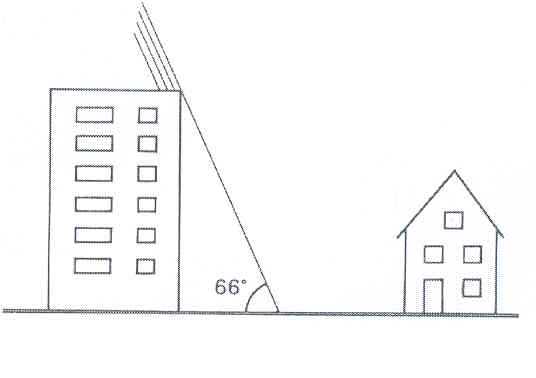
\includegraphics[width = 0.5\textwidth]{trigo/image/trigo11.png}
\end{center}
\end{exercice}

\begin{exercice}
La pente d’une route est de $12,5 \%$. Quel angle forment la route et l’horizontale ?
\end{exercice}

\begin{exercice}
Sur une carte à l’échelle 1 : 200, la distance entre les deux stations du funiculaire de Fribourg est de 55,9 cm (distance à vol d'oiseau). L’angle formé par les rails et l’horizontale mesure $22,88^\circ$. Calculer la pente moyenne et la distance parcourue par le funiculaire pour un aller et retour.
\begin{center}
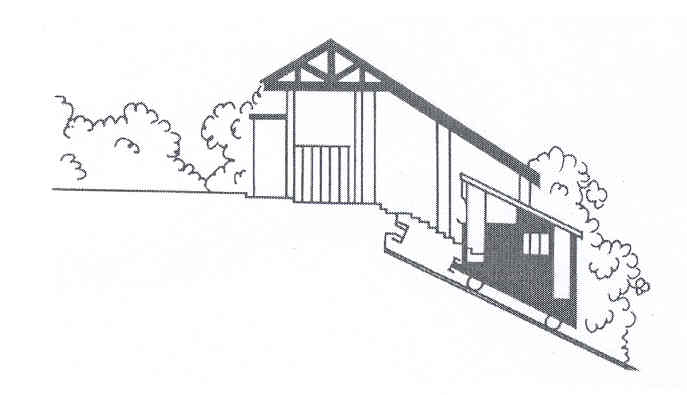
\includegraphics[width = 0.5\textwidth]{trigo/image/trigo13.png}
\end{center}
\end{exercice}

\begin{exercice}
Lorsque l’on se trouve sur le Vanil Noir, sous quel angle $\alpha $ aperçoit-on la Dent de Savigny ?
\begin{center}
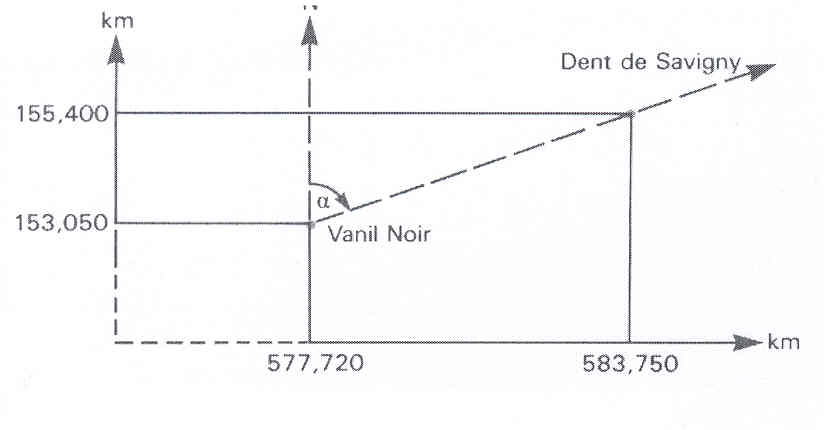
\includegraphics[width = 0.5\textwidth]{trigo/image/trigo14.png}
\end{center}
\end{exercice}

\begin{exercice}
De combien de mètres le ballon s’est-il élevé entre les deux mesures ?
$\begin{array}{l}
  c=780\text{ }m \\ 
 \alpha =65{}^\circ  \\ 
 \beta =73{}^\circ  \\ 
\end{array}$
\begin{center}
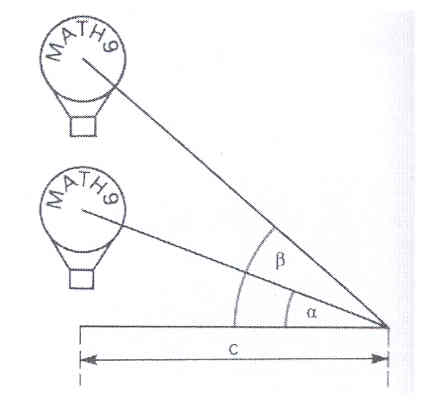
\includegraphics[width = 0.5\textwidth]{trigo/image/trigo15.png}
\end{center}
\end{exercice}

\begin{exercice}
Un observateur, éloigné de 15 m du pied E d'un pylône électrique vertical, vise le sommet S du pylône. Le point O de visée est situé à 1,6 m au-dessus du sol. L'angle formé par la droite (OS) et le plan horizontal mesure $35,4^\circ$. Quelle est la hauteur du pylône au-dessus du sol ?

\end{exercice}

\begin{exercice}
Calculer l'aire d'un triangle ABC, sachant que la hauteur issue de A mesure 4,89 m et qu'elle forme avec les côtés $\left[ AB \right]$ et $\left[ AC \right]$ des angles mesurant respectivement $8,3^\circ$ et $15,5^\circ$.

\end{exercice}

\begin{exercice}
Une route rectiligne fait un angle de $2,3^\circ$ par rapport à l'horizontale. Quel chemin faut-il parcourir pour s'élever de 110 mètres ?

\end{exercice}

\begin{exercice}
Voici un champ formé d'un trapèze rectangle et d'un triangle équilatéral.
\begin{center}
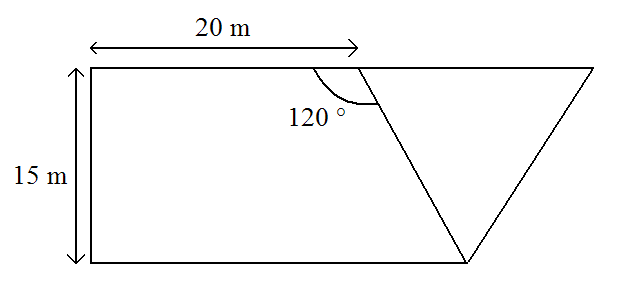
\includegraphics[width = 0.5\textwidth]{trigo/image/trigo19.png}
\end{center}
On désire ensemencer ce terrain de grains de blé, à raison de 0,80 kg par $m^2$. 

Quel sera le prix du blé à acheter si le kilogramme coûte Fr. 13.— ?

Quel est le rayon du cercle qui a le même périmètre que ce champ ? 
\end{exercice}
